% !TEX program = pdflatex
% Quantum Mechanics Homework_15
\documentclass[10pt,a4paper]{article}
\usepackage[margin=1in]{geometry} 
\usepackage{amsmath,amsthm,amssymb,amsfonts,enumitem,fancyhdr,color,comment,graphicx,environ}
\pagestyle{fancy}
\setlength{\headheight}{65pt}
\newenvironment{problem}[2][Problem]{\begin{trivlist}
\item[\hskip \labelsep {\bfseries #1}\hskip \labelsep {\bfseries #2.}]}{\end{trivlist}}
\newenvironment{sol}
    {\emph{Solution:}
    }
    {
    \qed
    }
\specialcomment{com}{ \color{blue} \textbf{Comment:} }{\color{black}}
\NewEnviron{probscore}{\marginpar{ \color{blue} \tiny Problem Score: \BODY \color{black} }}
\usepackage[UTF8]{ctex}
\usepackage{mathrsfs}
\usepackage{url}
\lhead{Name: 陈稼霖\\ StudentID: 45875852}
\rhead{PHYS1501 \\ Quantum Mechanics \\ Semester Fall 2019 \\ Assignment 15}
\begin{document}
\begin{problem}{1}
[C-T Exercise 13-1] Consider a one-dimensional harmonic oscillator of mass $m$, angular frequency $\omega_0$ and charge $q$. Let $|\varphi_n\rangle$ and $E_n=(n+\frac{1}{2})\hbar\omega_0$ be the eigenstates and eigenvalues of its Hamiltonian $\hat{H}_0$.\\
For $t<0$, the oscillator is in the ground state $|\varphi_0\rangle$. At $t=0$, it is subjected to an electric field "pulse" of duration $\tau$. The corresponding perturbation can be written $\hat{W}(t)=\left\{\begin{array}{ll}-q\mathscr{E}\hat{x},&0\leq t\leq\tau,\\0,&t<0,t>\tau\end{array}\right.$ Here $\mathscr{E}$ is the field amplitude and $\hat{x}$ and $\hat{x}$ is the position observerble. Let $\mathscr{P}(0n)$ be the probability of finding the oscillator in the state $|\varphi_n\rangle$ after the pulse.
\begin{itemize}
\item[(a)] Calculate $\mathscr{P}_{01}$ by using first-order time-dependent perturbation theory. How does $\mathscr{P}_{01}$ vary with $\tau$, for fixed $\omega_0$?
\item[(b)] Show that, to obtain $\mathscr{P}_{02}$, the time-dependent perturbation theory calculation must be pursued at least to second order. Calculate $\mathscr{P}_{02}$ to this perturbation order.
\end{itemize}
\end{problem}
\begin{sol}
\begin{itemize}
\item[(a)] Using first-order time-dependent perturbation theory, the probability of finding the oscillator in the state $|\varphi_n\rangle$ after the pulse is
\begin{equation}
\mathscr{P}_{01}=\frac{1}{\hbar^2}\left|\int_0^{t}dt'e^{i\omega_{10}t'}W_{10}(t')\right|^2
\end{equation}
where the upper bound of the integral $t>\tau$, the Bohr angular frequency between the initial state $|\varphi_0\rangle$ and the final state $|\varphi_1\rangle$ is
\begin{equation}
\omega_{10}=\frac{E_1-E_0}{\hbar}=\omega_0
\end{equation}
and the matrix element of the perturbation is
\begin{align}
\nonumber W_{10}(t)=&\langle\varphi_1|\hat{W}(t)|\varphi_0\rangle=\left\{\begin{array}{ll}
-q\mathscr{E}\langle\varphi_1|\hat{x}|\varphi_0\rangle,&0\leq t\leq\tau\\
0,&t<0,t>\tau
\end{array}\right.\\
\nonumber=&\left\{\begin{array}{ll}
-q\mathscr{E}\sqrt{\frac{\hbar}{2m\omega_0}}\langle\varphi_1|(\hat{a}+\hat{a}^{\dagger})|\varphi_0\rangle,&0\leq t\leq\tau\\
0,&t<0,t>\tau
\end{array}\right.\\
\nonumber=&\left\{\begin{array}{ll}
-q\mathscr{E}\sqrt{\frac{\hbar}{2m\omega_0}}\langle\varphi_1|\varphi_1\rangle,&0\leq t\leq\tau\\
0,&t<0,t>\tau
\end{array}\right.\\
=&\left\{\begin{array}{ll}
-q\mathscr{E}\sqrt{\frac{\hbar}{2m\omega_0}},&0\leq t\leq\tau\\
0,&t<0,t>\tau
\end{array}\right.
\end{align}
Therefore,
\begin{align}
\nonumber\mathscr{P}_{01}=&\frac{1}{\hbar^2}\left|-q\mathscr{E}\sqrt{\frac{\hbar}{2m\omega_0}}\int_0^{\tau}dt'e^{i\omega_0t}\right|^2\\
\nonumber=&\frac{1}{\hbar^2}\left|q\mathscr{E}\sqrt{\frac{\hbar}{2m\omega_0}}\frac{e^{i\omega_0\tau}-1}{\omega_0}\right|^2\\
\nonumber=&\frac{1}{\hbar^2}\left|q\mathscr{E}\sqrt{\frac{\hbar}{2m\omega_0}}\frac{e^{i\omega_0\tau/2}-e^{-i\omega_0\tau/2}}{\omega_0}\right|^2\\
\nonumber=&\frac{1}{\hbar^2}\left|q\mathscr{E}\sqrt{\frac{\hbar}{2m\omega_0}}\frac{2i\sin(\omega_0t/2)}{\omega_0}\right|^2\\
=&\frac{2q^2\mathscr{E}^2}{m\hbar\omega_0^3}\sin^2\left(\frac{\omega_0t}{2}\right)=\frac{q^2\mathscr{E}^2}{m\hbar\omega_0^3}\left(1-\cos\omega_0t\right)
\end{align}
$\mathscr{P}_{01}$ oscillates with $\tau$, for fixed $\omega_0$. When $t=\frac{2m\pi}{\omega_0}$, ($m=0,1,2,\cdots$), $\mathscr{P}_{01}$ reaches its maximum $\mathscr{P}_{01}=\frac{q\mathscr{E}}{m\hbar\omega^3}$, and when $t=\frac{(2m+1)\pi}{\omega_0}$, ($m=0,1,2,\cdots$), $\mathscr{P}_{01}$ reaches its minimum $\mathscr{P}_{01}=0$.
\item[(b)] We first calculate $\mathscr{P}_{02}$ to first order.
\begin{equation}
\mathscr{P}_{02}=\frac{1}{\hbar^2}\left|\int_0^tdt'e^{i\omega_{20}t'}W_{20}(t')\right|^2
\end{equation}
where the matrix element of $\hat{W}$ is
\begin{align}
\nonumber W_{20}(t)=&\langle\varphi_2|\hat{W}(t)|\varphi_0\rangle\\
\nonumber=&\left\{\begin{array}{ll}
-q\mathscr{E}\sqrt{\frac{\hbar}{2m\omega_0}}\langle\varphi_2|\varphi_1\rangle,&0\leq t\leq\tau\\
0,&t<0,t>\tau
\end{array}\right.\\
=&0
\end{align}
Therefore, to first order,
\begin{equation}
\mathscr{P}_{02}=0
\end{equation}
which means that
\begin{equation}
b_2(t)=b_2^{(0)}(t)+\lambda b_2^{(1)}(t)=0
\end{equation}
and
\begin{equation}
b_2^{(1)}(t)=0
\end{equation}
We must pursue the time-dependent perturbation theory calculation to the second order.
\begin{equation}
b_2(t)=b_2^{(0)}(t)+\lambda b_2^{(1)}(t)+\lambda^2b_2^{(2)}(t)
\end{equation}
The perturbation equation in the $2$nd order is
\begin{gather}
i\hbar\frac{d}{dt}b_2^{(2)}(t)=\sum_ke^{i\omega_{nk}t}W_{2k}(t)b_k^{(1)}(t)\\
\Longrightarrow i\hbar\frac{d}{dt}b_2^{(2)}=e^{i\omega_{20}t}W_{21}(t)b_1^{(1)}(t)\\
\Longrightarrow b_2^{(2)}(t)=b_2^{(2)}(0)+\frac{1}{i\hbar}\int_0^te^{i\omega_{21}}W_{21}b_1^{(1)}(t)=\frac{1}{i\hbar}\int_0^te^{i\omega_{21}t}W_{21}(t)b_1^{(1)}(t)
\end{gather}
The probability of finding the oscillator in the state $|\varphi_2\rangle$ is
\begin{equation}
\mathscr{P}_{20}(t)=|b_2(t)|^2=|b_2^{(2)}(t)|^2=\frac{1}{\hbar^2}\left|\int_0^tdt'e^{i\omega_{21}t'}W_{21}(t')b_1^{(1)}(t')\right|^2
\end{equation}
where $t>\tau$, the Bohr angular frequency between the state $|\varphi_2\rangle$ and $|\varphi_1\rangle$ is
\begin{equation}
\omega_{21}=\frac{E_2-E_1}{\hbar}=\omega_0
\end{equation}
the element of $\hat{W}$ is
\begin{align}
\nonumber\mathscr{P}_{21}=&\langle\varphi_2|\hat{W}(t)|\varphi_1\rangle\\
\nonumber=&\left\{\begin{array}{ll}
-q\mathscr{E}\sqrt{\frac{\hbar}{2m\omega_0}}\langle\varphi_2|\sqrt{2}|\varphi_2\rangle,&0\leq t\leq\tau\\
0,&t<0,t>\tau
\end{array}\right.\\
=&\left\{\begin{array}{ll}
-q\mathscr{E}\sqrt{\frac{\hbar}{m\omega_0}},&0\leq t\leq\tau\\
0,&t<0,t>\tau
\end{array}\right.
\end{align}
and
\begin{equation}
\mathscr{P}_{01}(t)=|b_1^{(1)}(t)|^2=\frac{q^2\mathscr{E}^2}{2m\hbar\omega_0^3}\left|e^{i\omega_0t}-1\right|^2\Longrightarrow b_1^{(1)}(t)=q\mathscr{E}\sqrt{\frac{1}{2m\hbar\omega_0^3}}(e^{i\omega_0t}-1)e^{i\phi_1}
\end{equation}
Therefore,
\begin{align}
\nonumber\mathscr{P}_{20}=&\frac{1}{\hbar^2}\left|-q\mathscr{E}\sqrt{\frac{\hbar}{m\omega_0}}q\mathscr{E}\sqrt{\frac{1}{2m\hbar\omega_0^3}}\int_0^{\tau}dt'e^{i\omega_0t'}(e^{i\omega_0t'}-1)\right|^2\\
\nonumber=&\frac{1}{\hbar^2}\left|\frac{q^2\mathscr{E}^2}{\sqrt{2}m\omega_0^2}\int_0^{\tau}dt'e^{2i\omega_0t'}-e^{i\omega_0t'}\right|^2\\
\nonumber=&\frac{1}{\hbar^2}\left|\frac{q^2\mathscr{E}^2}{\sqrt{2}m\omega_0^2}\left(\frac{e^{2i\omega_0\tau}-1}{2\omega_0}-\frac{e^{i\omega_0\tau}-1}{\omega_0}\right)\right|^2\\
=&\frac{q^2\mathscr{E}^2}{2m^2\hbar^2\omega_0^6}\left|\frac{e^{2i\omega\tau}}{2}-e^{i\omega_0\tau}+\frac{1}{2}\right|^2
\end{align}
\end{itemize}
\end{sol}

\begin{problem}{2}

[C-T Exercise 13-2] Consider two spin $1/2$'s, $\hat{\vec{S}}_1$ and $\hat{\vec{S}}_2$, coupled by an interaction of the form $a(t)\hat{\vec{S}}_1\cdot\hat{\vec{S}}_2$; $a(t)$ is a function of time which approaches zero when $|t|$ approaches infinity, and takes on non-negligible values (on the order of $a_0$) only inside an interval, whose width is of the order of $\tau$, about $t=0$.
\begin{itemize}
\item[(a)] At $t=-\infty$, the system is in the state $|+-\rangle$ (an eigenstate of $\hat{\vec{S}}_1$ and $\hat{\vec{S}}_2$ with the eigenvalues $\hbar/2$ and $-\hbar/2$). Calculate, without approximations, the state of the system at $t=+\infty$. Show that the probability $\mathscr{P}(+-\rightarrow-+)$ of finding, at $t=+\infty$, the system in the state $|-+\rangle$ depends only on the integral $\int_{-\infty}^{+\infty}dt~a(t)$.
\item[(b)] Calculate $\mathscr{P}(+-\rightarrow-+)$ by using first-order time-dependent perturbation theory. Discuss the validity conditions for such an approximation by comparing the results obtained with those of the preceding question.
\item[(c)] Now assume that the two spins are also interacting with a static magnetic field $\vec{B}_0$ parallel to $Oz$. The corresponding Zeeman Hamiltonian can be written $\hat{H}_0=-B_0(\gamma_1\hat{S}_{1z}+\gamma\hat{S}_{2z})$, where $\gamma_1$ and $\gamma_2$ are the gyromagnetic ratios of the two spins, assumed to be different.\\
Assume that $a(t)=a_0e^{-t^2/\tau^2}$. Calculate $\mathscr{P}(+-\rightarrow-+)$ by first-order time-dependent perturbation theory. With fixed $a_0$ and $\tau$, discuss the variation of $\mathscr{P}(+-\rightarrow-+)$ with respect to $B_0$.
\end{itemize}
\end{problem}
\begin{sol}
\begin{itemize}
\item[(a)] The initial state of the system can also be written as in the basis of $\{sm\}$
\begin{equation}
\label{2ini}
|\psi(t=-\infty)\rangle=|+-\rangle=\frac{1}{\sqrt{2}}[|00\rangle+|10\rangle]
\end{equation}
The coupling energy of the system in the state represented by the eigenvector $|sm\rangle$ in the basis $\{|sm\rangle\}$ is
\begin{gather}
\begin{align}
\nonumber\hat{W}(t)|sm\rangle=&a(t)\hat{\vec{S}}_1\cdot\hat{\vec{S}}_2|sm\rangle\\
\nonumber=&\frac{1}{2}a(t)(\hat{s}^2-\hat{s}_1^2-\hat{s}_2^2)|sm\rangle\\
=&\frac{1}{2}a(t)\hbar^2[s(s+1)-\frac{3}{2}]|sm\rangle
\end{align}\\
\Longrightarrow E_{sm}=\frac{1}{2}a(t)\hbar^2[s(s+1)-\frac{3}{2}]
\end{gather}
so $|sm\rangle$ is also an eigenvector of $W(t)$.\\
The Schrödinger equation is
\begin{equation}
i\hbar\frac{d|\psi\rangle}{dt}=\hat{W}|\psi\rangle
\end{equation}
\begin{equation}
i\hbar\frac{d}{dt}\sum_{s,m}c_{sm}(t)|sm\rangle=\hat{W}(t)\sum_{sm}c_{sm}(t)|sm\rangle
\end{equation}
\begin{equation}
\Longrightarrow i\hbar\frac{d}{dt}\sum_{s,m}c_{sm}(t)|sm\rangle=\frac{1}{2}a(t)\hbar^2\sum_{s,m}[s(s+1)-\frac{3}{2}]c_{sm}|sm\rangle
\end{equation}
\begin{equation}
\Longrightarrow i\hbar\frac{d}{dt}c_{sm}(t)=\frac{1}{2}a(t)\hbar^2[s(s+1)-\frac{3}{2}]c_{sm}
\end{equation}
\begin{equation}
\Longrightarrow \frac{\dot{c}_{sm}}{c_{sm}}=\frac{-i\hbar}{2}[s(s+1)-\frac{3}{2}]a(t)
\end{equation}
\begin{equation}
\Longrightarrow(\ln c_{sm})|_{-\infty}^{\infty}=\frac{-i\hbar}{2}[s(s+1)-\frac{3}{2}]\int_{-\infty}^{\infty}dta(t)
\end{equation}
\begin{equation}
c_{sm}(+\infty)=c_{sm}(-\infty)e^{\frac{-i\hbar}{2}[s(s+1)-\frac{3}{2}]\int_{-\infty}^{+\infty}dta(t)}
\end{equation}
Given the initial state as (\ref{2ini}), the final state of the system is
\begin{equation}
|\psi(t=+\infty)\rangle=\frac{1}{\sqrt{2}}(e^{\frac{3i\hbar}{4}}|00\rangle+e^{\frac{-i\hbar}{4}}|10\rangle)e^{\int_{-\infty}^{+\infty}dta(t)}
\end{equation}
Since $|+-\rangle$ can be written as in the basis of $\{|sm\rangle\}$
\begin{equation}
|+-\rangle=\frac{1}{\sqrt{2}}[|10\rangle-|00\rangle]
\end{equation}
The probability of finding, at $t=+\infty$, the system in the state $|-+\rangle$ is
\begin{align}
\nonumber\mathscr{P}(+-\rightarrow-+)=&\mathscr{P}(|\psi(+\infty)\rangle=|-+\rangle)=|\langle-+|\psi(+\infty)\rangle|^2\\
\nonumber=&\left|\frac{1}{\sqrt{2}}(-\langle00|+\langle10|)\frac{1}{\sqrt{2}}(e^{\frac{3i\hbar}{4}\int_{-\infty}^{+\infty}dta(a)}|00\rangle+e^{\frac{-i\hbar}{4}\int_{-\infty}^{+\infty}dta(t)}|10\rangle)\right|^2\\
=&\frac{1}{4}\left|(-e^{\frac{3i\hbar}{4}\int_{-\infty}^{+\infty}dta(t)}+e^{\frac{-i\hbar}{4}\int_{-\infty}^{+\infty}dta(t)})\right|^2
\end{align}
which depends only on the integral $\int_{-\infty}^{+\infty}dta(t)$.
\item[(b)] Using first-order time-dependent perturbation theory, the probability of finding, at $t=+\infty$, the system in the state $|-+\rangle$ is
\begin{equation}
\mathscr{P}(+-\rightarrow-+)=\frac{1}{\hbar^2}\left|\int_{-\infty}^{+\infty}dte^{i\omega_{fi}t}W_{fi}(t)\right|^2
\end{equation}
where the Bohr angular frequency between the initial state and the state $|-+\rangle$
\begin{equation}
\omega_{fi}=\frac{E_f-E_i}{\hbar}=0
\end{equation}
and the matrix element of $\hat{W}$ is
\begin{align}
\nonumber\hat{W}_{fi}(t)=&\langle-+|\hat{W}(t)|+-\rangle\\
\nonumber=&\frac{1}{\sqrt{2}}[-\langle00|+\langle10|]\hat{W}(t)\frac{1}{\sqrt{2}}[|00\rangle+|10\rangle]\\
\nonumber=&\frac{1}{4}a(t)\hbar^2[-\langle00|+\langle10|][-\frac{3}{2}|00\rangle+\frac{1}{2}|10\rangle]\\
=&\frac{1}{2}\hbar^2a(t)
\end{align}
Therefore,
\begin{equation}
\mathscr{P}(+-\rightarrow-+)=\frac{\hbar^2}{4}\left|\int_{-\infty}^{+\infty}dta(t)\right|^2
\end{equation}
Span $\mathscr{P}(+-\rightarrow-+)$ obtain from (a) about $\int_{-\infty}^{+\infty}dta(t)=0$ and obtain the higher order terms, we can get
\begin{equation}
\mathscr{P}(+-\rightarrow-+)=\frac{1}{4}\left|(-e^{\frac{3i\hbar}{4}\int_{-\infty}^{+\infty}dta(t)}+e^{\frac{-i\hbar}{4}\int_{-\infty}^{+\infty}dta(t)})\right|^2=\frac{\hbar^2}{4}\left|\int_{-\infty}^{+\infty}dta(t)\right|^2+O\left(\left|\int_{-\infty}^{+\infty}dta(t)\right|^3\right)
\end{equation}
which is the same as the result obtain in (b) above. Therefore, such an approximation to first order is valid when $\left|\int_{-\infty}^{+\infty}dta(t)\right|^2$
\item[(c)] In the static magnetic field, the energy of the initial state is
\begin{align}
\nonumber E_{+-}=&\langle+-|\hat{H}_0|+-\rangle\\
\nonumber=&\langle+-|(-B_0)(\gamma_1\hat{S}_{1z}+\gamma_2\hat{S}_{2z})|+-\rangle\\
\nonumber=&-B_0\langle+-|(\gamma_1\frac{\hbar}{2}-\gamma_2\frac{\hbar}{2})|+-\rangle\\
=&-B_0(\gamma_1-\gamma_2)\frac{\hbar}{2}
\end{align}
the energy of the state $|-+\rangle$ is
\begin{equation}
\nonumber E_{-+}=\langle-+|\hat{H}_0|-+\rangle=-B_0(-\gamma_1+\gamma_2)\frac{\hbar}{2}
\end{equation}
The Bohr angular frequency between the two states above is
\begin{equation}
\omega_{fi}=\frac{E_{-+}-E_{+-}}{\hbar}=B_0(\gamma_1-\gamma_2)
\end{equation}
The matrix element of $\hat{W}(t)$ is
\begin{equation}
\hat{W}_{fi}(t)=\frac{1}{2}\hbar^2a_0e^{-t^2/\tau^2}
\end{equation}
Therefore,
\begin{align}
\nonumber\mathscr{P}(+-\rightarrow-+)=&\frac{1}{\hbar^2}\left|\int_{-\infty}^{+\infty}dte^{iB_0(\gamma_1-\gamma_2)t}\frac{1}{2}\hbar^2a_0e^{-t^2/\tau^2}\right|^2\\
\nonumber=&\frac{\hbar^2|a_0|^2}{4}\left|\int_{-\infty}^{+\infty}e^{-t^2/\tau^2+iB_0(\gamma_1-\gamma_2)}\right|^2\\
\nonumber=&\frac{\hbar^2|a_0|^2}{4}\left|e^{-\left[\frac{B_0(\gamma_1-\gamma_2)\tau}{2}\right]^2}\int_{-\infty}^{+\infty}e^{-\frac{1}{\tau^2}\left[t-\frac{iB_0(\gamma_1-\gamma_2)\tau}{2}\right]^2}\right|^2\\
\nonumber=&\frac{\hbar^2|a_0|^2}{4}\left|e^{-\left[\frac{B_0(\gamma_1-\gamma_2)\tau}{2}\right]^2}\int_{-\infty}^{+\infty}\sqrt{\pi}\tau\right|^2\\
=&\frac{\pi^2\hbar^2|a_0|^2\tau^2}{4}e^{-\frac{B_0^2(\gamma_1-\gamma_2)^2\tau^2}{2}}
\end{align}
$\mathscr{P}(+-\rightarrow-+)$ decreases exponentially as $B_0$ increases.
\end{itemize}
\end{sol}

\begin{problem}{3}
A particle of mass $\mu$ is scattered by the central field $V(r)=\frac{\alpha}{r^2}$ with $\alpha>0$. Find the differential and total scattering cross section under the first-order Born approximation.
\end{problem}
\begin{sol}
Under the first-order Born approximation, the differential scattering cross section is
\begin{align}
\nonumber\frac{d\sigma_k^{(B)(\theta,\phi)}}{d\Omega}=&\frac{\mu^2}{4\pi^2\hbar^4}\left|\int d^3re^{-i\vec{q}\cdot\vec{r}}V(\vec{r})\right|^2\\
\nonumber=&\frac{\mu^2}{4\pi^2\hbar^4}\left|\int d^3re^{-i\vec{q}\cdot\vec{r}}\alpha r^{-2}\right|^2\\
\nonumber=&\frac{\mu^2}{4\pi^2\hbar^4}\left|\int_0^{+\infty}dr'r^{'2}\int_{-1}^{+1}d(\cos\theta')\int_0^{2\pi}d\phi e^{-2ikr'\sin(\theta/2)\cos\theta'}\alpha r^{'-2}\right|^2\\
\nonumber=&\frac{\mu^2}{4\pi^2\hbar^4}\left|2\pi\alpha\int_0^{+\infty}dr'\int_{-1}^{+1}d(\cos\theta')e^{-2ikr'\sin(\theta/2)\cos\theta'}\right|^2\\
\nonumber=&\frac{\mu^2}{4\pi^2\hbar^4}\left|2\pi\alpha\int_0^{+\infty}dr'\frac{-2i\sin[2kr'\sin(\theta/2)]}{-2kr'\sin(\theta/2)}\right|^2\\
\nonumber=&\frac{\mu^2}{4\pi^2\hbar^4}\left|\frac{2\alpha\pi}{k\sin(\theta/2)}\int_0^{+\infty}d[2kr'\sin(\theta/2)]\frac{\sin[2kr'\sin(\theta/2)]}{2kr'\sin(\theta/2)}\right|^2\\
\nonumber&(\text{let }2kr'\sin(\theta/2)=\xi)\\
\nonumber=&\frac{\mu^2}{4\pi^2\hbar^4}\left|\frac{2\alpha\pi}{k\sin(\theta/2)}\int_0^{+\infty}d\xi\frac{\sin\xi}{\xi}\right|^2\\
\nonumber=&\frac{\mu^2}{4\pi^2\hbar^4}\left|\frac{2\alpha\pi}{k\sin(\theta/2)}\frac{\pi}{2}\right|^2\\
=&\frac{\pi^2\alpha^2\mu^2}{4\hbar^4k^2\sin^2(\theta/2)}
\end{align}
The total scattering cross section is
\begin{align}
\nonumber\sigma_t=&\int d\Omega\frac{d\sigma(\theta,\phi)}{d\Omega}\\
\nonumber=&\int_{-1}^{+1}d(\cos\theta)\int_0^{2\pi}d\phi\frac{\pi^2\alpha^2\mu^4}{4\hbar^4k^2\sin^2(\theta/2)}\\
\nonumber=&\frac{2\pi^3\alpha^2\mu^4}{4\hbar^4k^2\sin^2(\theta/2)}\int_{-1}^{+1}d(\cos\theta)\frac{1}{\sin^2(\theta/2)}\\
\nonumber=&\frac{2\pi^3\alpha^2\mu^4}{4\hbar^4k^2\sin^2(\theta/2)}\int_{-1}^{+1}d(\cos\theta)\frac{2}{1-\cos\theta}\\
\nonumber=&\frac{2\pi^3\alpha^2\mu^4}{4\hbar^4k^2\sin^2(\theta/2)}\left[-2\ln(1-\cos\theta)\right]_{\cos\theta=-1}^{+1}\\
=&\infty
\end{align}
\end{sol}

\begin{problem}{4}
[C-T Complement C$_\text{VIII}$-3 Exercise b] Consider a central potential $V(r)$ such that $V=\left\{\begin{array}{ll}-V_0,&r<r_0,\\0,&r>0.\end{array}\right.$ Here $V_0$ is a positive constant. Set $k_0=\sqrt{2\mu V_0/\hbar^2}$ with $\mu$ the mass of the particle subject to the potential. We shall confine ourselves to the study of the $s$ wave ($l=0$).
\begin{itemize}
\item[(a)] Bound states ($E<0$)]
\begin{itemize}
\item[i.] Write the radial equation in the two regions $r>r_0$ and $r<r_0$, as well as the condition at the origin. Show that, if one sets $\rho=\sqrt{-2\mu E/\hbar^2}$ and $K=\sqrt{k_0^2-\rho^2}$, the function $u_0(r)$ is necessarily of the form $u_0(r)=\left\{\begin{array}{ll}Ae^{-\rho r},&r>r_0\\B\sin(Kr),&r<r_0\end{array}\right.$
\item[ii.] Write the matching conditions at $r=R_0$. Deduce from them that the only possible values for $\rho$ are those which satisfy the equation $\tan(Kr_0)=-K/\rho$.
\item[iii.] Discuss the equation $\tan(Kr_0)=-K/\rho$. Indicate the number of $s$ bound states as a function of the depth of the well (for fixed $r_0$) and show, in particular, that there are no bound states if this depth is too small. 
\end{itemize}
\item[(b)] Scattering resonances ($E>0$)]
\begin{itemize}
\item[i.] Again write the radial equation, this time setting $k=\sqrt{2\mu E/\hbar}$ and $K'=\sqrt{k_0^2+k^2}$. Show that $u_{k,0}(r)$ is of the form $u_{k,0}=\left\{\begin{array}{ll}A\sin(kr+\delta_0),&r>r_0,\\B\sin(K'r),&r<r_0.\end{array}\right.$
\item[ii.] Choosing $A=1$. Show, using the continuity conditions aT $r=r_0$, that the constant $B$ and the phase shift $\delta_0$ are given by $B^2=k^2/[k^2+k_0^2\cos^2(K'r_0)]$ and $\delta_0=-kr_0+\alpha(k)$ with $\tan\alpha(k)=(k/K')\tan(K'r_0)$.
\item[iii.] Trace the curve representing $B^2$ as a function of $k$. This curve clearly shows resonances, for which $B^2$ is maximum. What are the values of $k$ associated with these resonances? What is then the value of $\alpha(k)$? Show that, if there exists such a resonance for a small energy ($kr_0\ll1$), the corresponding contribution of the $s$ wave to the total cross section is practically maximal.
\end{itemize}
\item[(c)] Relation between bound states and scattering resonances\\
Assume that $k_0r_0$ is very close to $(2n+1)\pi/2$, where $n$ is an integer, and set $k_0r_0=(2n+1)\pi/2+\varepsilon$ with $|\varepsilon|\ll1$.
\begin{itemize}
\item[i.] Show that, if $\varepsilon$ is positive, there exists a bound state whose binding energy $E=-\hbar^2\rho^2/2\mu$ is given by $\rho\approxeq\varepsilon k_0$.
\item[ii.] Show that if, on the other hand, $\varepsilon$ is negative, there exists a scattering resonance at energy $E=\hbar^2k^2/2\mu$ such that $k^2\approxeq-2k_0\varepsilon/r_0$.
\item[iii.] Deduce from this that if the depth of the well is gradually decreased (for fixed $r_0$), the bound state which disappears when $k_0r_0$ passes through an odd multiple of $\pi/2$ gives rise to a low energy scattering resonance.
\end{itemize}
\end{itemize}
\end{problem}
\begin{sol}
\begin{itemize}
\item[(a)]
\begin{itemize}
\item[i.] The stationary state wave functions in the central potential can be written as
\begin{equation}
\varphi_{klm}(\vec{r})=R_{kl}(r)Y_{lm}(\theta,\phi)=\frac{u_{kl}(r)}{r}Y_lm(\theta,\phi)
\end{equation}
The general radical equation is
\begin{equation}
\left[-\frac{\hbar^2}{2\mu}\frac{d^2}{dr^2}+\frac{l(l+1)}{2\mu r^2}+V(r)\right]u_{kl}(r)=\frac{\hbar^2k^2}{2\mu}u_{kl}(r)
\end{equation}
Confined to $s$ wave (l=0), in the region $r>r_0$,
\begin{equation}
\label{r>r0}
\left[\frac{d^2}{dr^2}-\rho^2\right]u_{k0}(r)=0,\quad r>r_0
\end{equation}
and in the region $r<r_0$,
\begin{gather}
\label{r<r0}
\left[\frac{d^2}{dr^2}+K^2\right]u_{k0}(r)=0,\quad r<r_0
\end{gather}
The general solution to equation (\ref{r>r0}) is
\begin{equation}
u_{k0}(r)=A_+e^{\rho r}+A_-e^{-\rho r},\quad r>r_0
\end{equation}
Considering the boundary condition,
\begin{gather}
\lim_{r\rightarrow\infty}(r)\rightarrow0\\
\Longrightarrow A_+=0
\end{gather}
so relabel $A_-$ as $A$,
\begin{equation}
u_{k0}(r)=Ae^{-\rho r},\quad r>r_0
\end{equation}
The general solution to equation (\ref{r<r0}) is
\begin{equation}
u_{k0}(r)=B_+e^{iKr}+B_-e^{-iKr},\quad r<r_0
\end{equation}
Considering the condition at the origin,
\begin{equation}
u_{k0}(r)=0\\
\Longrightarrow B_+=-B_-=B
\end{equation}
so
\begin{equation}
u_{k0}(r)=B\sin Kr,\quad r<r_0
\end{equation}
\item[ii.] The matching conditions at $r=r_0$ are
\begin{gather}
B\sin Kr_0=Ae^{-\rho r_0}\\
BK\cos Kr_0=-\rho Ae^{-\rho r_0}
\end{gather}
Dividing the two equations above, we get
\begin{equation}
\tan Kr_0=-\frac{K}{\rho}
\end{equation}
\item[iii.] The number of $s$ bound states is equal to the number of the intersection of the curve $y(K)=\tan Kr_0$ and $y(k)=-\frac{K}{\rho}=-\frac{1}{\sqrt{\frac{k_0^2}{J}-1}}$ as shown in figure \ref{problem_41}, where $0<K<k_0$ due to $-V<E<0$ for bound states.
\begin{figure}[h]
\centering
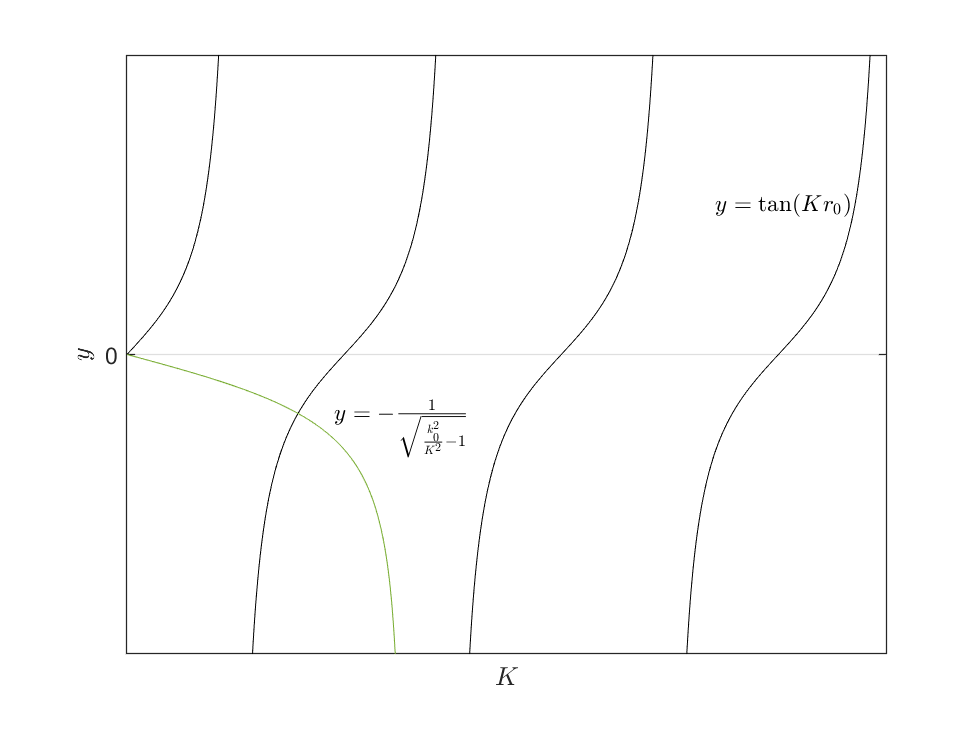
\includegraphics[width=.5\textwidth]{problem_41.png}
\caption{Problem 5 (a) iii.}\label{problem_41}
\end{figure}
\\The number of intersections of the two curves within $(0,k_0)$ is
\begin{equation}
n=\left\lceil\frac{k_0}{\pi/r_0}-\frac{1}{2}\right\rceil=\left\lceil\frac{\sqrt{2\mu V_0/\hbar^2}}{\pi/r_0}-\frac{1}{2}\right\rceil
\end{equation}
If $k_0\leq\frac{\pi}{2r_0}$, the two curves do not have any intersection within $(0,k_0)$.\\
\end{itemize}
\item[(b)]
\begin{itemize}
\item[i.] In the region $r>r_0$, the radical equation is
\begin{equation}
\label{r>r02}
\left[\frac{d^2}{dr^2}+k^2\right]u_{k0}(r)=0,\quad r>r_0
\end{equation}
In the region $r<r_0$, the radical equation is
\begin{equation}
\label{r<r02}
\left[\frac{d^2}{dr^2}+K'^2\right]u_{k0}(r)=0,\quad r<r_0
\end{equation}
The general solution to (\ref{r>r02}) is
\begin{equation}
u_{k0}(r)=A_+e^{ikr}+A_-e^{-ikr},\quad r>r_0
\end{equation}
The setting of scattering resonance is equivalent to a one-dimensional problem with $V(r)=\infty$ for $r<0$, in which $|A_-|^2$ is the amplitude of the incident plane wave and $|A_+|^2$ is the amplitude of the reflected plane wave at large $r$. Since there is no transmission, we have
\begin{gather}
|A_+|^2=|A_-|^2\\
\Longrightarrow u_{k0}(r)=A(e^{ikr}e^{i\phi_+}+e^{-ikr}e^{i\phi_-})=A\sin(kr+\delta_0),\quad r>r_0
\end{gather}
The general solution to equation (\ref{r<r02}) is
\begin{equation}
u_{k0}=B_+e^{iK'r}+B_-e^{iK'r},\quad r<r_0
\end{equation}
Considering the condition at origin,
\begin{equation}
u_{k0}(0)=0
\end{equation}
we have
\begin{equation}
B_+=B_-=\frac{B}{2}
\end{equation}
so
\begin{equation}
u_{k0}(r)=B\sin(K'r),\quad r<r_0
\end{equation}
Therefore,
\begin{equation}
u_{k0}(r)=\left\{\begin{array}{ll}A\sin(kr+\delta_0),&r>r_0,\\B\sin(K'r),&r<r_0.\end{array}\right.
\end{equation}
\item[ii.] The matching conditions at $r=r_0$ are
\begin{gather}
\sin(kr_0+\delta_0)=B\sin(K'r_0)\\
k\cos(kr_0+\delta_0)=BK'\cos(K'r_0)
\end{gather}
Square the two equations above, we get
\begin{gather}
\sin^2(kr_0+\delta_0)=B^2\sin^2(K'r_0)\\
\cos^2(kr_0+\delta_0)=B^2\frac{K^{'2}}{k^2}\cos(K'r_0)
\end{gather}
Add the two equations above, we get
\begin{gather}
1=B^2\left[\sin^2(K'r_0)+\frac{K^{'2}}{k^2}\cos^2(K'r_0)\right]\\
\Longrightarrow B^2=\frac{1}{\left[1-\cos^2(K'r_0)+\frac{K^{'2}}{k^2}\cos^2(K'r_0)\right]}\\
\Longrightarrow B^2=\frac{k^2}{k^2+k_0^2\cos^2(K'r_0)}
\end{gather}
Devide the two equations at the beginning, we get
\begin{equation}
\tan(kr_0+\delta_0)=\frac{k}{K'}\tan(K'r_0)
\end{equation}
Using $\delta_0=-kr_0+\alpha(k)$, we get
\begin{equation}
\tan\alpha(k)=\frac{k}{K'}\tan(K'r_0)
\end{equation}
\item[iii.] The minima occur at $\cos^2(K'r_0)=0$ or
\begin{gather}
K'r_0=\sqrt{k_0^2+k^2}=\frac{(2n+1)\pi}{2r_0}\\
k=\sqrt{\left(\frac{(2n+1)\pi}{2r_0}\right)^2-k_0^2}
\end{gather}
where $n$ is integer.\\
At these values of $k$, $\tan(K'r_0)$ blows up, as does $\tan\alpha(k)$, so
\begin{equation}
\alpha(k)=(m+\frac{1}{2})\pi
\end{equation}
where $m$ is integer.\\
The total cross section is
\begin{equation}
\sigma=\frac{4\pi}{k^2}\sum_{l=0}^{\infty}(2l+1)\sin^2\delta_l
\end{equation}
For $kr_0\ll1$, at resonace
\begin{align}
\nonumber\sin^2\delta_0=&\sin^2(-kr_0+\alpha(k))\\
\nonumber=&\sin^2\left(-kr_0+(m+\frac{1}{2})\pi\right)\\
\nonumber=&\left[(-1)^m\cos kr_0\right]^2\\
\nonumber=&\cos^2kr_0\\
=&1-(kr_0)^2+O[(kr_0)^4]
\end{align}
Therefore, $\sin\delta_0$ is practically maximal.
\end{itemize}
\item[(c)]
\begin{itemize}
\item[i.] Guess $\rho\approx\varepsilon k_0$ when $k_0r_0=(n+\frac{1}{2})\pi+\varepsilon$ with $\varepsilon$ positive and $\varepsilon\ll1$,
\begin{align}
\nonumber\tan(Kr_0)=&\tan\sqrt{k_0^2-\rho^2}r_0\\
\nonumber=&\tan\left[(1-\varepsilon^2)^{1/2}\left((n+\frac{1}{2})\pi+\varepsilon\right)\right]\\
\nonumber=&\tan\left[(1-\frac{1}{2}\varepsilon^2+O(\varepsilon^4))\left((n+\frac{1}{2})\pi+\varepsilon\right)\right]\\
\nonumber=&\tan\left[(n+\frac{1}{2})\pi+O(\varepsilon^2)\right]\\
\nonumber=&-\cot\left[\varepsilon+O(\varepsilon^2)\right]\\
\nonumber=&-\frac{\cos\left[\varepsilon+O(\varepsilon^2)\right]}{\sin\left[\varepsilon+O(\varepsilon^2)\right]}\\
\nonumber=&-\frac{1-\frac{1}{2}\varepsilon^2+O(\varepsilon^3)}{\varepsilon}\\
=&-\frac{1}{\varepsilon}+\frac{1}{2}\varepsilon+O(\varepsilon^2)
\end{align}
\begin{align}
\nonumber-\frac{K}{\rho}=&-\frac{\sqrt{k_0^2-\rho^2}}{\rho}\\
\nonumber=&-\frac{1-\varepsilon^2}{\varepsilon}\\
\nonumber=&-\frac{1-\frac{1}{2}\varepsilon^2+O(\varepsilon^3)}{\varepsilon}\\
=&-\frac{1}{\varepsilon}+\frac{1}{2}\varepsilon+O(\varepsilon^2)
\end{align}
\begin{equation}
\Longrightarrow\tan(Kr_0)=-\frac{K}{\rho}
\end{equation}
so the guess is correct.
\item[ii.] The resonance condition is
\begin{equation}
k^2=\left((n+\frac{1}{2})\frac{\pi}{r_0}\right)^2-k_0^2
\end{equation}
Plug $k_0=\frac{1}{r_0}[(n+\frac{1}{2})\frac{\pi}{2}+\varepsilon]$ into the equation above, we get
\begin{align}
\nonumber k^2=&\left((n+\frac{1}{2})\frac{\pi}{r_0}\right)-\frac{1}{r_0^2}\left[(n+\frac{1}{2})\pi+\varepsilon\right]^2\\
\nonumber=&\left((n+\frac{1}{2})\frac{\pi}{r_0}\right)^2-\frac{1}{r_0^2}\left((n+\frac{1}{2})\pi\right)^2-\frac{2\varepsilon}{r_0^2}\left((n+\frac{1}{2})\pi\right)-\frac{\varepsilon^2}{r_0^2}\\
\nonumber=&-\frac{2\varepsilon}{r_0^2}\left((n+\frac{1}{2})\pi\right)-\frac{\varepsilon^2}{r_0^2}\\
\nonumber=&-\frac{2k_0\varepsilon}{r_0}+O(\varepsilon^2)
\end{align}
\item[iii.] When the depth of the well is gradually decreased or $k_0$ gradually decreased and $k_0r_0$ pass through an odd multiple of $\frac{\pi}{2}$, one of the intersections in figure \ref{problem_41} disappears and resonance appears in (ii) at about the same energy.
\end{itemize}
\end{itemize}
\small{Reference: \url{https://phys.cst.temple.edu/~meziani/homework2s_5702_2017.pdf}}
\end{sol}

\begin{problem}{5}
[C-T Exercise 14-3] Consider the state space of an electron, spanned by the two vectors $|\varphi_{p_x}\rangle$ and $|\varphi_{p_y}\rangle$ which represent two atomic orbitals, $p_x$ and $p_y$, of wave functions $\varphi_{p_x}(\vec{r})$ and $\varphi_{p_y}(\vec{r})$, $\varphi_{p_x}(\vec{r})=xf(r)=rf(r)\sin\theta\cos\phi$, $\varphi_{p_y}(\vec{r})=yf(r)=rf(r)\sin\theta\sin\phi$.
\begin{itemize}
\item[(a)] Write, in terms of $|\varphi_{p_x}\rangle$ and $|\varphi_{p_y}\rangle$, the state $|\varphi_{p_{\alpha}}\rangle$ which represents the $p_{\alpha}$ orbital pointing in the direction of the $xOy$ plane which makes an angle $\alpha$ with $Ox$.
\item[(b)] Consider two electrons whose spins are both in the $|+\rangle$ state, the eigenstate of $\hat{S}_z$ of eigenvalue $+\hbar/2$. Write the normalized state vector $|\psi\rangle$ which represents the system of two electrons, one of which is in the state $|\varphi_{p_x}\rangle$ and the other in the state $|\varphi_{p_y}\rangle$.
\item[(c)] Same question, with one of the electrons in the state $|\varphi_{p_{\alpha}}\rangle$ and the other one in the state $|\varphi_{p_{\beta}}\rangle$, where $\alpha$ and $\beta$ are two arbitrary angles. Show that the state vector $|\psi\rangle$ obtained is the same.
\item[(d)] The system is in the state $|\psi\rangle$ of question (b). Calculate the probability density $\mathscr{P}(r,\theta,\phi;r',\theta',\phi)$ of finding one electron at $(r,\theta,\phi)$ and the other one at $(r',\theta',\phi')$. Show that the electronic density $\rho(r,\theta,\phi)$ [the probability density of finding any electron at $(r,\theta,\phi)$] is symmetrical wich respect to revolution about the $Oz$ axis. Determine the probability density of having $\phi-\phi'=\phi_0$, where $\phi_0$ is given. Discuss the variation of this probability density with respect to $\phi_0$.
\end{itemize}
\end{problem}
\begin{sol}
\begin{itemize}
\item[(a)] The state which represents the $p_{\alpha}$ orbital pointing in the direction of the $xOy$ plane which makes an angle $\alpha$ with $Ox$ is
\begin{equation}
|\varphi_{p_{\alpha}}\rangle=\cos\alpha|\varphi_{p_{x}}\rangle+\sin\alpha|\varphi_{p_y}\rangle
\end{equation}
\item[(b)] The state vector which represents the system of two electrons, one of which is in the state $|\varphi_{p_x}\rangle$ and the other in the state $|\varphi_{p_y}\rangle$ is
\begin{equation}
|\psi_{12}\rangle=\frac{1}{\sqrt{2}}\left|\begin{array}{cc}
|\psi_1\rangle&|\psi_1\rangle\\
|\psi_2\rangle&|\psi_2\rangle\\
\end{array}\right|=\frac{1}{\sqrt{2}}(|\psi_1\rangle|\psi_2\rangle-|\psi_2\rangle|\psi_1\rangle)
\end{equation}
where
\begin{gather}
|\psi_1\rangle=|\varphi_{p_x}\rangle\otimes|+\rangle\\
|\psi_2\rangle=|\varphi_{p_y}\rangle\otimes|+\rangle
\end{gather}
Therefore,
\begin{equation}
|\psi_{12}\rangle=\frac{1}{\sqrt{2}}(|\varphi_{p_x}\varphi_{p_y}\rangle-|\varphi_{p_y}\varphi_{p_x}\rangle)|++\rangle
\end{equation}
\item[(c)] Let
\begin{gather}
|\psi_1\rangle=(\cos\alpha|\varphi_{p_x}\rangle+\sin\alpha|\varphi_{p_y}\rangle)\otimes|+\rangle\\
|\psi_2\rangle=(\cos\beta|\varphi_{p_x}\rangle+\sin\beta|\varphi_{p_y}\rangle)
\end{gather}
For simplicity, write
\begin{equation}
|+\rangle=\alpha(s_i)
\end{equation}
where $i=1$ or $2$ depending on the particle.
\begin{align}
\nonumber\psi_1(\vec{r}_1,s_1)\psi_2(\vec{r}_2,s_2)=&\alpha(s_1)\alpha(s_2)(\cos\alpha\varphi_{p_x}(\vec{r}_1)+\sin\alpha\varphi_{p_y}(\vec{r}_1))(\cos\beta\varphi_{p_x}(\vec{r}_2)+\sin\beta\varphi_{p_y}(\vec{r}_2))\\
\nonumber=&\alpha(s_1)\alpha(s_2)[\cos\alpha\cos\beta\varphi_{p_x}(\vec{r}_1)\varphi_{p_x}(\vec{r}_2)+\cos\alpha\sin\beta\varphi_{p_x}(\vec{r}_1)\varphi_{p_y}(\vec{r}_2)\\
&+\sin\alpha\cos\beta\varphi_{p_y}(\vec{r}_1)\varphi_{p_x}(\vec{r}_2)+\sin\alpha\sin\beta\varphi_{p_y}(\vec{r}_1)\varphi_{p_y}(\vec{r}_2)]
\end{align}
and
\begin{align}
\nonumber\psi_2(\vec{r}_1,s_1)\psi_1(\vec{r}_2,s_2)=&\alpha(s_1)\alpha(s_2)(\cos\beta\varphi_{p_x}(\vec{r}_1)+\sin\beta\varphi_{p_y}(\vec{r}_1))(\cos\alpha\varphi_{p_x}(\vec{r}_2)+\sin\alpha\varphi_{p_y}(\vec{r}_2))\\
\nonumber=&\alpha(s_1)\alpha(s_2)[\cos\beta\cos\alpha\varphi_{p_x}(\vec{r}_1)\varphi_{p_x}(\vec{r}_2)+\cos\beta\sin\alpha\varphi_{p_x}(\vec{r}_1)\varphi_{p_y}(\vec{r}_2)\\
&+\sin\beta\cos\alpha\varphi_{p_y}(\vec{r}_1)\varphi_{p_x}(\vec{r}_2)+\sin\beta\sin\alpha\varphi_{p_y}(\vec{r}_1)\varphi_{p_y}(\vec{r}_2)]
\end{align}
Therefore,
\begin{align}
\nonumber|\psi_{12}\rangle=&\frac{1}{\sqrt{2}}(|\psi_1\rangle|\psi_2\rangle-|\psi_2\rangle|\psi_1\rangle)|++\rangle\\
\nonumber=&\frac{1}{\sqrt{2}}[\varphi_{p_x}(\vec{r}_1)\varphi_{p_y}(\vec{r}_2)(\cos\alpha\sin\beta-\cos\beta\sin\alpha)+\varphi_{p_y}(\vec{r}_1)\varphi_{p_x}(\vec{r}_2)(\sin\alpha\cos\beta-\cos\alpha\sin\beta)]|++\rangle\\
\nonumber=&\frac{1}{\sqrt{2}}[\varphi_{p_x}(\vec{r}_1)\varphi_{p_y}(\vec{r}_2)-\varphi_{p_y}(\vec{r}_1)\varphi_{p_x}(\vec{r}_2)]|++\rangle\sin(\beta-\alpha)
\end{align}
After normalization,
\begin{equation}
|\psi_{12}\rangle=\frac{1}{\sqrt{2}}[\varphi_{p_x}(\vec{r}_1)\varphi_{p_y}(\vec{r}_2)-\varphi_{p_y}(\vec{r}_1)\varphi_{p_x}(\vec{r}_2)]|++\rangle
\end{equation}
which is the same as the result obtained in (b).
\item[(d)] Since we are not to observe the spin, the spin part of the state vector can be hidden.
\begin{gather}
|\psi_{12}\rangle=\frac{1}{\sqrt{2}}[\varphi_{p_x}(\vec{r}_1)\varphi_{p_y}(\vec{r}_2)-\varphi_{p_y}(\vec{r}_1)\varphi_{p_x}(\vec{r}_2)]\\
\begin{align}
\Longrightarrow\psi_{12}(r,\theta,\phi;r',\theta',\phi')=&\frac{1}{\sqrt{2}}rr'f(r)f(r')\sin\theta\sin\theta'(\cos\phi\sin\phi'-\sin\phi\cos\phi')\\
=&\frac{1}{\sqrt{2}}rr'f(r)f(r')\sin\theta\sin\theta'\sin(\phi'-\phi)
\end{align}
\end{gather}
The probability density of finding one electron at $(r,\theta,\phi)$ and the other one at $(r',\theta',\phi')$ is
\begin{align}
\nonumber\mathscr{P}(r,\theta,\phi;r',\theta',\phi')=&\langle\psi_{12}|\psi_{12}\rangle\\
\nonumber=&|\psi_{12}(r,\theta,\phi;r',\theta',\phi')|^2r^2r^{'2}\sin\theta\sin\theta'\\
\nonumber=&\frac{1}{2}r^4r^{'4}|f(r)|^2|f(r')|^2\sin^4\theta\sin^4\theta'\sin^2(\phi'-\phi)\\
=&F(r,\theta;r',\theta')\sin^2(\phi'-\phi)
\end{align}
The electron density is
\begin{equation}
\rho(r,\theta,\phi)=\int_0^{+\infty}r^2dr\int_0^{\pi}\sin\theta'd\theta'\int_0^{2\pi}d\phi'\mathscr{P}(r,\theta,\phi;r',\theta',\phi')
\end{equation}
When we rotate with respect to $z$ axis
\begin{gather}
\phi\rightarrow\phi+\phi_0\\
\phi'\rightarrow\phi'+\phi_0
\end{gather}
The probability density becomes
\begin{align}
\nonumber\mathscr{P}(r,\theta,\phi+\phi_0;r',\theta',\phi'+\phi_0)=&F(r,\theta;r',\theta')\sin^2[(\phi'+\phi_0)-(\phi+\phi_0)]\\
\nonumber=&F(r,\theta;r',\theta')\sin^2(\phi'-\phi)\\
=&\mathscr{P}(r,\theta,\phi;r',\theta',\phi')
\end{align}
The probability density is symmetrical to revolution about the $Oz$ axis, so the electron density is also symmetrical to revolution about the $Oz$.\\
When $\phi-\phi'=\phi_0$, the this probability density is
\begin{equation}
\mathscr{P}(r,\theta,\phi;r',\theta',\phi')=F(r,\theta;r',\theta')\sin^2(\phi_0)\propto\sin^2(\phi_0)
\end{equation}
\end{itemize}
\end{sol}
\end{document}